\documentclass[a4]{article}

% PAQUETES %%%%%%%%%%%%%%%%%%%%%%%%%%%%%%%%%%%%%%%%%%%%%%%%%%%%%%%%%%%%%%%%%%%%%
\usepackage[utf8]{inputenc}
\usepackage{framed} % Para crear cuadros alrededor del texto
\usepackage{makecell}
\usepackage[english]{babel}
%
\usepackage[fixlanguage]{babelbib}
    \bibliographystyle{IEEEtran}

\usepackage{url}

%!TEX encoding = UTF-8 Unicode
% !TEX spellcheck = es

\setlength{\textwidth}{6.5 in}
\setlength{\textheight}{8.5 in}
\setlength{\headsep}{0.5 in}

\usepackage{multirow, array} % para las tablas
\usepackage{float} % para usar [H]
\usepackage{charter}

\usepackage[breaklinks=true]{hyperref}

%
% ADD PACKAGES here:
%

\usepackage[utf8]{inputenc}
\usepackage{amsmath,longtable,siunitx, float, graphicx, dcolumn, bm, fancyhdr, authblk, subcaption, caption, hyperref, multicol, setspace}

\usepackage{bbding}
\usepackage{amssymb}
\usepackage[rightcaption]{sidecap}
%\usepackage{textcomp}

\usepackage[hmarginratio=1:1, top=32mm, columnsep=20pt, headsep=\dimexpr20mm, margin=0.7in, top=1in ]{geometry}

\usepackage{booktabs}
\usepackage{multirow}

\usepackage{algorithm}
\usepackage{enumitem}
\usepackage{tabularx}
\usepackage[noend]{algpseudocode}
\usepackage{xcolor}

\usepackage{tikz}
\usetikzlibrary{shapes.geometric, arrows.meta, positioning}

% ----------- global styles -----------
\tikzset{
  font=\scriptsize,                      % tiny text everywhere
  every node/.style       = {transform shape},   % respect scale
  startstop/.style        = {ellipse, draw, fill=blue!10,
                             inner sep=1pt, minimum width=13mm},
  process/.style          = {rectangle, draw, fill=orange!15,
                             text width=26mm, inner sep=2pt, align=center},
  decision/.style         = {diamond, draw, fill=green!15, aspect=2.3,
                             text width=20mm, inner sep=1pt, align=center},
  arrow/.style            = {->, >=Stealth, shorten >=1pt, shorten <=1pt}
}

\newcommand{\TODO}{\textbf{\textcolor{red}{TODO}}}

\renewcommand{\algorithmicrequire}{\textbf{Input:}}
\renewcommand{\algorithmicensure}{\textbf{Output:}}

\lhead{\includegraphics[scale=0.4]{CETC.png}}
\rhead{\includegraphics[scale=0.025]{Cornell-University-Logo.png}}

\newtheorem{theo}{Theorem}
\newenvironment{theorem}
  {\begin{mdframed}\begin{theo}}
  {\end{theo}\end{mdframed}}
  
\newtheorem{prop}{Proposición}
\newenvironment{proposition}
  {\begin{mdframed}\begin{prop}}
  {\end{prop}\end{mdframed}}

\newtheorem{lem}{Lema}
\newenvironment{lema}
  {\begin{mdframed}\begin{lem}}
  {\end{lem}\end{mdframed}}
  
\newtheorem{defi}{Definition}
\newenvironment{definition}
  {\begin{mdframed}\begin{def}}
  {\end{def}\end{mdframed}}
  
\newtheorem{proof}{Proof}
\newtheorem{remark}{Remark}

\usepackage[numbers]{natbib}
\renewcommand{\thesection}{\Roman{section}}
%\setlength{\parskip}{\baselineskip}%

\begin{document}

\thispagestyle{fancy}

\begin{center}
    \textbf{\large Orbit Odyssey - Computer Vision} \\
    {Field Definition}
    
    \vspace{0.7em}

    David Alejandro Fuquen \\

    {\small \today}

\end{center}

\section*{Playing Field Definition}

\subsection*{Summary}
This part of Phase 1 defines all the structure, positions, conditions and specifications for the playing field. This is the first part of the competition manual. For this case, we will consider the partition of the original field can't be taken away. 


\section*{Field dimensions, boundaries and markings}
We will use the same dimensions and boundaries as the original Space Odyssey. The same 4x8 field will be used, while maintaining the inner field partition. 

The playing field is a rectangular arena enclosed by low-profile PVC pipe barriers on all four sides, with a central partition dividing it into two halves.

\begin{table}[H]
\centering
\begin{tabular}{ll}
\toprule
\textbf{Property} & \textbf{Value} \\
\midrule
Total length (X-axis) & 254.00 cm (100 in) \\
Total width (Y-axis) & 142.24 cm (56 in) \\
Total floor area & 3.61 m\textsuperscript{2} \\
Perimeter walls & Low-profile PVC pipe barriers \\
Corner zones & 30.48 $\times$ 30.48 cm (12 $\times$ 12 in) at each corner \\
Partition & \textbf{Present} --- see below \\
\bottomrule
\end{tabular}
\caption{Field dimensions and boundaries.}
\end{table}

\subsubsection*{Central partition}

\begin{table}[H]
\centering
\begin{tabular}{ll}
\toprule
\textbf{Property} & \textbf{Value} \\
\midrule
Orientation & Horizontal, centered on both axes \\
Y-axis position & Y = 71.12 cm (28 in) --- midpoint of field width \\
Length & 127.00 cm (50 in) --- half the field length \\
X-axis span & X = 63.50 cm to X = 190.50 cm \\
Left gap & X = 0 to 63.50 cm (25 in wide) \\
Right gap & X = 190.50 to 254.00 cm (25 in wide) \\
Height & Same as perimeter walls (low PVC pipe --- camera sees over it) \\
\bottomrule
\end{tabular}
\caption{Central partition specifications.}
\end{table}

The coordinate system places the origin $(0, 0)$ at the bottom-left corner of the field. The X-axis runs left to right (0 to 254 cm) and the Y-axis runs bottom to top (0 to 142.24 cm). The partition does \textbf{not} block the camera's line of sight (the camera sits above pipe height). It only blocks the robot's driving path through the center 50 inches, forcing it to navigate around via the 25-inch gaps on either side.

\begin{figure}[H]
\centering
\begin{tikzpicture}
  \begin{scope}[scale=0.055]
    \draw[thick] (0,0) rectangle (254, 142.24);
    \draw[dashed, blue!60] (0,0) rectangle (30.48, 30.48);
    \draw[dashed, blue!60] (254-30.48,0) rectangle (254, 30.48);
    \draw[dashed, blue!60] (0,142.24-30.48) rectangle (30.48, 142.24);
    \draw[dashed, blue!60] (254-30.48,142.24-30.48) rectangle (254, 142.24);
    % Partition
    \draw[very thick, orange!80!black] (63.50, 71.12) -- (190.50, 71.12);
    % Objects
    \filldraw[red!70!black] (45.72, 45.72) circle (6);
    \filldraw[red!70!black] (127.00, 25.40) circle (6);
    \filldraw[red!70!black] (208.28, 45.72) circle (6);
    \filldraw[red!70!black] (83.82, 96.52) circle (6);
    \filldraw[red!70!black] (170.18, 116.84) circle (6);
    % Zigzag connections
    \draw[dashed, gray!50] (45.72,45.72) -- (127.00,25.40) -- (208.28,45.72);
    \draw[dashed, gray!50] (45.72,45.72) -- (83.82,96.52);
    \draw[dashed, gray!50] (208.28,45.72) -- (170.18,116.84);
    \draw[<->, >=Stealth] (0,-12) -- (254,-12);
    \draw[<->, >=Stealth] (-12,0) -- (-12,142.24);
  \end{scope}
  \node[font=\footnotesize\bfseries, anchor=east] at (2.18,2.51) {\textsf{P1}};
  \node[font=\footnotesize\bfseries, anchor=north] at (6.99,1.06) {\textsf{P2}};
  \node[font=\footnotesize\bfseries, anchor=west] at (11.79,2.51) {\textsf{P3}};
  \node[font=\footnotesize\bfseries, anchor=south] at (4.61,5.64) {\textsf{P4}};
  \node[font=\footnotesize\bfseries, anchor=south] at (9.36,6.76) {\textsf{P5}};
  \node[font=\scriptsize, orange!80!black, anchor=south] at (6.99,4.10) {Partition};
  \node[blue!70, font=\scriptsize] at (0.84,0.84) {LRZ};
  \node[blue!70, font=\scriptsize] at (13.13,0.84) {LRZ};
  \node[blue!70, font=\scriptsize] at (0.84,6.98) {LRZ};
  \node[blue!70, font=\scriptsize] at (13.13,6.98) {LRZ};
  \node[font=\footnotesize] at (6.99,-1.10) {254 cm (100 in)};
  \node[font=\footnotesize, rotate=90] at (-1.21,3.91) {142.24 cm (56 in)};
  \node[font=\scriptsize, anchor=north east] at (-0.11,-0.11) {$(0,0)$};
\end{tikzpicture}
\caption{Layout P\_5 --- zigzag pattern, 3 bottom + 2 top (partition present).}
\end{figure}

//TODO (David): Add an image with the field. DON'T DO THIS, I'll do it myself.

\section*{Robot starting zone and placement rules}
The Robot will start in any of the two corners known as \textit{Low Rubble Zone} in the original orbit Odyssey. So long the robot is within the boundaries of that corner, the team may decide where the robots points to. Ideally, this will be the only human-made decision of the challenge, the only part in which the team has any kind of decision-making ablities. 

\section*{Object quantity, placement templates, and clearance constraints}
\subsection*{Object count and class breakdown}
This layout uses \textbf{5 objects}: 1 Rocket (contact) + 2 Tires (avoid) + 2 Tin Cans (avoid). Each object has an approximate radius of 6 cm. The objects are split across both halves of the field (\textbf{3 bottom, 2 top}) and arranged in a \textbf{high-low-high zigzag} pattern: side objects sit closer to the partition, center objects closer to the outer wall. This prevents the robot from getting boxed in by a horizontal line of objects.

\subsection*{Object positions}

\begin{table}[H]
\centering
\begin{tabular}{clccccc}
\toprule
\textbf{ID} & \textbf{Location} & \textbf{X (in)} & \textbf{Y (in)} & \textbf{X (cm)} & \textbf{Y (cm)} & \textbf{Half} \\
\midrule
P1 & Left gap lane, near partition & 18 & 18 & 45.72 & 45.72 & Bottom \\
P2 & Center, near bottom wall & 50 & 10 & 127.00 & 25.40 & Bottom \\
P3 & Right gap lane, near partition & 82 & 18 & 208.28 & 45.72 & Bottom \\
P4 & Behind partition, left & 33 & 38 & 83.82 & 96.52 & Top \\
P5 & Near top wall, right & 67 & 46 & 170.18 & 116.84 & Top \\
\bottomrule
\end{tabular}
\caption{Object positions --- Layout P\_5 (zigzag).}
\end{table}

\subsection*{Clearance verification}

\textbf{Minimum clearances:} object center to wall $\geq$ 20 cm, object center to partition $\geq$ 20 cm, object center to object center $\geq$ 35 cm, objects must be outside all corner zones.

\begin{table}[H]
\centering
\begin{tabular}{cccccc}
\toprule
\textbf{ID} & \textbf{Min wall (cm)} & \textbf{Partition (cm)} & \textbf{In gap lane?} & \textbf{Nearest obj. (cm)} \\
\midrule
P1 & 45.7 (left) \checkmark & 25.4 \checkmark & Yes ($X < 63.5$) & 64 (P4) \checkmark \\
P2 & 25.4 (bottom) \checkmark & 45.7 \checkmark & Under partition & 84 (P1) \checkmark \\
P3 & 45.7 (right) \checkmark & 25.4 \checkmark & Yes ($X > 190.5$) & 81 (P5) \checkmark \\
P4 & 83.8 (left) \checkmark & 25.4 \checkmark & Behind partition & 64 (P1) \checkmark \\
P5 & 25.4 (top) \checkmark & 45.7 \checkmark & Behind partition & 81 (P3) \checkmark \\
\bottomrule
\end{tabular}
\caption{Clearance verification.}
\end{table}

\subsection*{Distance from each corner to each object (cm)}

\begin{table}[H]
\centering
\begin{tabular}{lccccc}
\toprule
\textbf{Corner} & \textbf{P1} & \textbf{P2} & \textbf{P3} & \textbf{P4} & \textbf{P5} \\
\midrule
Bottom-Left & \textbf{43} & 112 & 195 & 106 & 185 \\
Bottom-Right & 195 & 112 & \textbf{43} & 175 & 123 \\
Top-Left & 87 & 151 & 210 & \textbf{75} & 155 \\
Top-Right & 210 & 151 & 87 & 158 & \textbf{69} \\
\bottomrule
\end{tabular}
\caption{Distance from each corner zone center to each object position.}
\end{table}

\subsection*{Navigation notes}

The camera sees all 5 objects from any corner (the low partition does not block vision). The partition only affects the driving path:

\begin{itemize}
    \item \textbf{From bottom corners:} P1, P2, P3 are directly reachable. P4 and P5 require going around the partition via the left gap ($X < 63.5$ cm) or right gap ($X > 190.5$ cm).
    \item \textbf{From top corners:} P4 and P5 are directly reachable. P1, P2, P3 require going around.
    \item \textbf{Zigzag prevents trapping:} the robot always has a clear lane between the staggered objects.
    \item \textbf{Estimated detour per crossing:} $\sim$5--10 seconds depending on position relative to nearest gap.
\end{itemize}

\subsection*{Suggested class rotation templates}

Positions are physically fixed. Between heats, the referee assigns classes to positions.

\subsubsection*{Option A: ``Dodge First'' (robot starts on bottom half)}

\begin{table}[H]
\centering
\begin{tabular}{lccccc}
\toprule
\textbf{Template} & \textbf{P1} & \textbf{P2} & \textbf{P3} & \textbf{P4} & \textbf{P5} \\
\midrule
A1 & Tire & Tin Can & Tire & \textbf{Rocket} & Tin Can \\
A2 & Tin Can & Tire & Tin Can & \textbf{Rocket} & Tire \\
\bottomrule
\end{tabular}
\caption{``Dodge First'' templates --- bottom half is all avoid objects.}
\end{table}

\subsubsection*{Option B: Balanced}

\begin{table}[H]
\centering
\begin{tabular}{lccccc}
\toprule
\textbf{Template} & \textbf{P1} & \textbf{P2} & \textbf{P3} & \textbf{P4} & \textbf{P5} \\
\midrule
B1 & \textbf{Rocket} & Tire & Tin Can & Tire & Tin Can \\
B2 & Tire & \textbf{Rocket} & Tin Can & Tire & Tin Can \\
\bottomrule
\end{tabular}
\caption{Balanced templates --- contact target on the start side.}
\end{table}






\end{document}
